% !TEX encoding = UTF-8
% !TEX TS-program = pdflatex
% !TEX root = ../tesi.tex

%**************************************************************
\chapter{Verifica e validazione}
\label{cap:verifica}
La \textbf{verifica} e \textbf{validazione} di un prodotto software hanno lo scopo di accertare che esso rispecchi i requisiti e che li rispetti nella maniera dovuta. Con l’attività di \textbf{verifica} viene accertato che lo stato di avanzamento del prodotto soddisfi i requisiti precedentemente fissati. Grazie a questa attività è possibile accertare la corretta costruzione del software. L’attività di \textbf{validazione} ha invece lo scopo di accertare che il prodotto finale corrisponda alle attese in modo da soddisfare tutti i requisiti prefissati in fase di analisi.\\ \\
Durante il mio stage lo sviluppo delle nuove funzionalità ha portato alla minimizzazione dei tempi di verifica e validazione. Tale decisione è stata presa in comune accordo con il tutor aziendale, in quanto lo scopo dello stage mirava all’estensione di più funzionalità possibili, che potranno essere testate successivamente dall’azienda.
Questa decisione è inoltre appoggiata dalla metodologia \emph{agile} utilizzata nello sviluppo del progetto, la quale definisce la qualità del software come la capacità di soddisfare i bisogni del cliente piuttosto che soddisfare metriche fissata a priori.
In ogni caso, vista l'importanza di queste attività, sono state adottate tecniche di analisi statica e analisi dinamica per il codice sorgente, al fine di verificarne e validarne il comportamento.
\begin{itemize}
	\item \textbf{analisi statica}: l'analisi statica è il processo di valutazione di un sistema o di un suo componente basato sulla sua forma, struttura, contenuto, documentazione senza che esso sia eseguito. Gli strumenti di analisi statica del codice consentono di individuare porzioni di codice del proprio programma ad alta probabilità di errore. Avendo a disposizione una lista di linee di codice sospette, un programmatore può poi verificare se siano presenti errori e, in caso positivo, rivedere il codice corrispondente e correggere le problematiche individuate;
	\item \textbf{analisi dinamica}: l'analisi dinamica è il processo di valutazione di un sistema software o di un suo componente basato sulla osservazione del suo comportamento in esecuzione.
\end{itemize}


\section{Verifica e validazione dei chatbots}
Gran parte del progetto di stage verteva nell'istruire gli \emph{agent} di api.ai per gestire le domande degli utenti fatte attraverso i \gls{Chatbot}. Essendo quindi una parte molto importante del prodotto sono stati creati alcuni test per verificare e validare le sue funzionalità. Questi test non sono stati automatizzati in quanto si è deciso di svolgerli attraverso due pagine Facebook create dall'azienda dove sono stati associati i due \glspl{Chatbot} di prova.\\
Si è quindi pensato insieme al tutor di impostare una serie di domande da porre al bot, cercando di coprire tutti i requisiti che esso dovesse soddisfare. \\
Grazie a questi controlli è stato possibile accertare che entrambi i \glspl{Chatbot} soddisfano tutti i requisiti obbligatori e desiderabili esposti nella sezione \ref{requisiti}.\\ \\
La procedura seguita per verificare e validare il comportamento dei due \glspl{Chatbot} è stata la seguente:
\begin{itemize}
	\item decisione della domanda da sottoporre in base ai requisiti da soddisfare;
	\item previsione della risposta che il \gls{Chatbot} doveva fornire;
	\item scrittura della domanda tramite la chat di Facebook o Messenger;
	\item controllo della risposta; nel caso fosse sbagliata:
	\begin{itemize}
		\item scrittura della domanda nella sezione dedicata di api.ai per verificare che il \gls{JSON} ritornato fosse corretto;
		\item correzione della logica di api.ai nel caso fosse sbagliata la risposta;
		\item controllo e correzione del codice nel caso il \gls{JSON} fosse corretto.
	\end{itemize}
\end{itemize}	 
Questa procedura viene rappresentata nel seguente diagramma di flusso.

\begin{figure}[t]
	\centering
	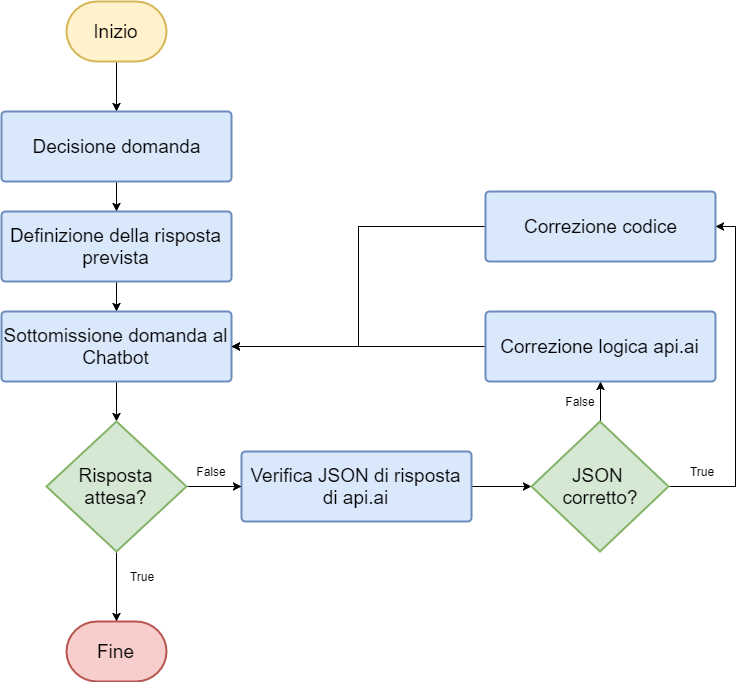
\includegraphics[scale=0.5]{../Immagini/verifica.png}
	\caption{Flowchart del processo di verifica dei chatbots}
\end{figure}

